\documentclass[
    % -- opções da classe memoir --
    article,			% indica que é um artigo acadêmico
    11pt,				% tamanho da fonte
    oneside,			% para impressão apenas no recto. Oposto a twoside
    a4paper,			% tamanho do papel. 
    % -- opções da classe abntex2 --
    %chapter=TITLE,		% títulos de capítulos convertidos em letras maiúsculas
    %section=TITLE,		% títulos de seções convertidos em letras maiúsculas
    %subsection=TITLE,	% títulos de subseções convertidos em letras maiúsculas
    %subsubsection=TITLE % títulos de subsubseções convertidos em letras maiúsculas
    % -- opções do pacote babel --
    english,			% idioma adicional para hifenização
    brazil,				% o último idioma é o principal do documento
    sumario=tradicional
]{abntex2}

% Pacotes
% -----
% Pacotes fundamentais 
% -----
\usepackage{lmodern}			% Usa a fonte Latin Modern
\usepackage[T1]{fontenc}		% Seleção de códigos de fonte.
\usepackage[utf8]{inputenc}		% Codificação do documento (conversão automática dos acentos)
\usepackage{indentfirst}		% Identa o primeiro parágrafo de cada seção.
\usepackage{nomencl} 			% Lista de símbolos
\usepackage{color}				% Controle das cores
\usepackage{graphicx}			% Inclusão de gráficos
\usepackage{microtype} 			% Para melhorias de justificação
\usepackage[brazilian,hyperpageref]{backref}	 % Páginas com as citações na bibliografia
\usepackage[subentrycounter,seeautonumberlist,nonumberlist=true,acronym,nohypertypes={acronym}]{glossaries} % Glossário. Deve ser carregado depois de backref
\usepackage[alf]{abntex2cite}	% Citações padrão ABNT. Deve ser carregado depois de glossaries
\usepackage[portuguese]{todonotes}
% -----

% -----
% Configurações dos pacotes
% -----

% --- Glossaries ---
\makeglossaries{} % Habilite este comando para permitir a impressão dos glossários
\loadglsentries{glossaries}
\renewcommand*{\glsclearpage}{} % Evita quebra de página entre os glossários

% --- Backref ---
% Usado sem a opção hyperpageref de backref
\renewcommand{\backrefpagesname}{Citado na(s) página(s):~}
% Texto padrão antes do número das páginas
\renewcommand{\backref}{}
% Define os textos da citação
\renewcommand*{\backrefalt}[4]{
    \ifcase #1 %
        Nenhuma citação no texto.%
    \or
        Citado na página #2.%
    \else
        Citado #1 vezes nas páginas #2.%
    \fi}%

% --- Todonotes ---
\setlength{\marginparwidth}{2cm}
\presetkeys{todonotes}{inline,backgroundcolor=yellow}{}

% -----

% Definições do trabalho
% -----
% Informações de dados para CAPA e FOLHA DE ROSTO
% -----
\titulo{DCC067 Computação Evolucionista: Trabalho Prático 1 --- Avaliação do uso de seleção por roleta e por torneio com variações de K e avaliação do uso de crossover de um ponto e aritmético}
\tituloestrangeiro{DCC067 Evolutionary Computing: Practical Work 1 --- Evaluation of the use of roulette and tournament selection with variations of K and evaluation of the use of one-point and arithmetic crossover}

\autor{%
    Celso Gabriel Malosto \and
    Lucas Paiva Santos \and
    Victor Duque Pinto
}

\local{Juiz de Fora}
\data{\glsentrydesc{dcc}, \glsentrydesc{ufjf}\newline2024}
% -----

% Configurações do documento
% -----
% Configurações de aparência do PDF final
% -----
\definecolor{blue}{RGB}{41,5,195}
% Informações do PDF
\makeatletter
\hypersetup{%
    %pagebackref=true,
    pdftitle={\@title},
    pdfauthor={\@author},
    pdfsubject={Modelo de artigo científico com abnTeX2},
    pdfcreator={LaTeX with abnTeX2},
    pdfkeywords={abnt}{latex}{abntex}{abntex2}{artigo científico},
    colorlinks=true,       		% false: boxed links; true: colored links
    linkcolor=blue,          	% color of internal links
    citecolor=blue,        		% color of links to bibliography
    filecolor=magenta,      		% color of file links
    urlcolor=blue,
    bookmarksdepth=4
}
\makeatother
% -----

% -----
% Demais configurações
% -----

% Compila o índice
\makeindex

% Altera as margens padrões
\setlrmarginsandblock{3cm}{3cm}{*}
\setulmarginsandblock{3cm}{3cm}{*}
\checkandfixthelayout{}

% Espaçamentos entre linhas e parágrafos
\setlength{\parindent}{1.3cm} % Tamanho do parágrafo
\setlength{\parskip}{0.2cm}  % Controle do espaçamento entre um parágrafo e outro
\SingleSpacing{} % Espaçamento simples

% -----

% Início do documento
\begin{document}

% -----
% Configurações do texto
% -----
% Seleciona o idioma do documento
\selectlanguage{brazil}

% Retira espaço extra obsoleto entre as frases
\frenchspacing{}
% -----

% =====
% ELEMENTOS PRÉ-TEXTUAIS
% =====
\pretextual{}

% Página de titulo principal (obrigatório)
\maketitle{}

% Resumos
% Resumo em português
\begin{resumoumacoluna}
    Conforme a ABNT NBR 6022:2018, o resumo no idioma do documento é elemento obrigatório.
    Constituído de uma sequência de frases concisas e objetivas e não de uma
    simples enumeração de tópicos, não ultrapassando 250 palavras, seguido, logo
    abaixo, das palavras representativas do conteúdo do trabalho, isto é,
    palavras-chave e/ou descritores, conforme a NBR 6028. (\ldots) As
    palavras-chave devem figurar logo abaixo do resumo, antecedidas da expressão
    Palavras-chave:, separadas entre si por ponto e finalizadas também por ponto.

    \vspace{\onelineskip}

    \noindent
    \textbf{Palavras-chave}: latex. abntex. editoração de texto.
\end{resumoumacoluna}

% Resumo em inglês
\renewcommand{\resumoname}{Abstract}
\begin{resumoumacoluna}
    \begin{otherlanguage*}{english}
        According to ABNT NBR 6022:2018, an abstract in foreign language is optional.

        \vspace{\onelineskip}

        \noindent
        \textbf{Keywords}: latex. abntex.
    \end{otherlanguage*}
\end{resumoumacoluna}


\begin{center}\smaller{}
    \textbf{Data de submissão e aprovação}: 28 de agosto de 2024.
\end{center}
% =====

% =====
% ELEMENTOS TEXTUAIS
% =====
\textual{}

\section{Introdução}%
\label{sec:introducao}

Este trabalho é requisito parcial para aprovação na disciplina \gls{disciplina}, do \gls{dcc} da \gls{ufjf}.

Seu objetivo é analisar a performance de \glspl{ga} ao encontrar soluções para problemas de otimização, em particular, a convergência e a qualidade das soluções encontradas.

Nesse sentido, o escopo do trabalho é avaliar
o uso de seleção por roleta e por torneio com variações de \(K\) --- a proporção de indivíduos selecionados para o torneio ---, além de avaliar o uso de \gls{crossover} de um ponto e aritmético.

Para tal, foi desenvolvido um projeto na linguagem Python, a fim de executar experimentos computacionais.
Como referência, foram utilizados classes de funções objetivo do \gls{cec14}, disponibilizadas pelo pacote \gls{opfunu}, que contém funções de benchmark para otimização~\cite{opfunu_paper}.
Além disso, foi utilizada a classe \gls{esga} da biblioteca \gls{mealpy}, que contém implementações de diversos algoritmos evolutivos~\cite{mealpy_paper}.

Com o código em operação, decidiu-se explorar as funções disponibilizadas pelo pacote, com o objetivo de selecionar uma função convexa e outra não convexa, que serviram como objetos de estudo no experimento.

O restante deste trabalho está organizado da seguinte forma: a \autoref{sec:metodologia} descreve a metodologia utilizada para a realização dos experimentos; a \autoref{sec:resultados} apresenta os resultados obtidos; e a \autoref{sec:conclusao} apresenta as conclusões do trabalho.


\section{Metodologia}%
\label{sec:metodologia}

A fim de conduzir este trabalho, foi realizada uma pesquisa bibliográfica sobre \glspl{ga} e suas variações, o que possibilitou a compreensão do funcionamento desses algoritmos e a identificação de aspectos relevantes para a análise de sua performance.
Assim, foram escolhidas duas funções de benchmark dentre as disponíveis no pacote \gls{opfunu}~\cite{opfunu_software}, uma convexa e outra não convexa.

\subsection{Operadores}

O objetivo central desta pesquisa é avaliar diferentes operadores de seleção e \gls{crossover}, com a intenção de entender como essas variações impactam os resultados dos experimentos.
Para isso, foram escolhidos os seguintes operadores de seleção: roleta e torneio --- que foi testado com diferentes valores de \(K\), que representa a proporção de indivíduos selecionados para o torneio dentre a totalidade da população.
Além disso, foram escolhidos os operadores de \gls{crossover} de um ponto e aritmético.

Embora inicialmente o escopo do trabalho não contemplasse a introdução de mutações, foi necessário incluir alguma chance de mutação para evitar problemas de convergência prematura das soluções, o que poderia limitar significativamente a qualidade dos resultados obtidos.

Assim, foram realizados testes preliminares com diferentes métodos de mutação disponíveis no pacote \gls{mealpy}~\cite{mealpy_software}.
Os resultados desses revelaram que algumas técnicas, como \texttt{scramble} e \texttt{inverted}, eram incompatíveis com certas combinações de operadores --- como a combinação de seleção por roleta com crossover de um ponto.

Em contraste, a mutação do tipo \texttt{flip} mostrou-se bastante razoável em termos de tempo de execução e resultados obtidos, independentemente da combinação de operadores utilizada (roleta, torneio, crossover de um ponto e crossover aritmético).
Dessa forma, foi selecionada a mutação \texttt{flip} em todas as execuções do experimento.

\subsection{Funções objetivo}

Ademais, foi necessário ultrapassar os limites do escopo originalmente estabelecido também no que se refere ao número de dimensões avaliadas.
O objetivo inicial era analisar as funções em 2 e 10 dimensões, o que não constitui uma limitação da biblioteca \gls{mealpy}.
Entretanto, os arquivos que baseiam o pacote \gls{opfunu} apresentam as funções objetivo disponíveis em apenas cinco configurações: 10, 20, 30, 50 e 100 dimensões.

Levando em conta que se esperava que as execuções para duas dimensões permitissem a visualização gráfica do espaço de busca delimitado pelas funções, e que tal artefato não pôde ser gerado pelo software, foram inclusos os gráficos gerados por \citeonline{cec2014}.
Dessa forma, optou-se por avaliar as funções em 10 e 20 dimensões, que são os valores mais próximos daqueles inicialmente planejados.

As duas funções objetivo escolhidas para a realização dos experimentos foram \gls{f1}, que é convexa e cuja representação gráfica é apresentada na \autoref{fig:f1}, e \gls{f5}, que é não convexa e cuja representação gráfica é apresentada na \autoref{fig:f5}.

\begin{figure}[!ht]%
    \centering
    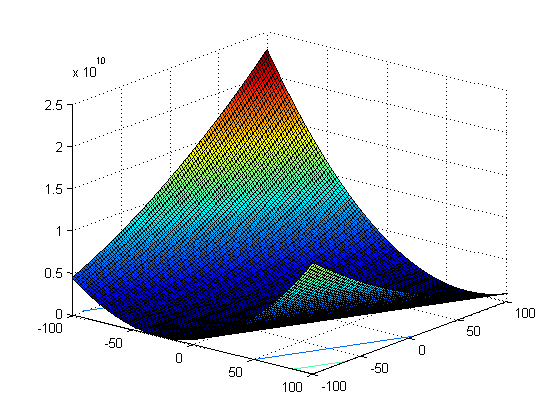
\includegraphics[scale=0.5]{img/f1.png}
    \caption{Mapa 3D para a função \glsentryfull{f1} em duas dimensões. Fonte: \citeonline{cec2014}.}%
    \label{fig:f1}
\end{figure}

\begin{figure}[!ht]%
    \centering
    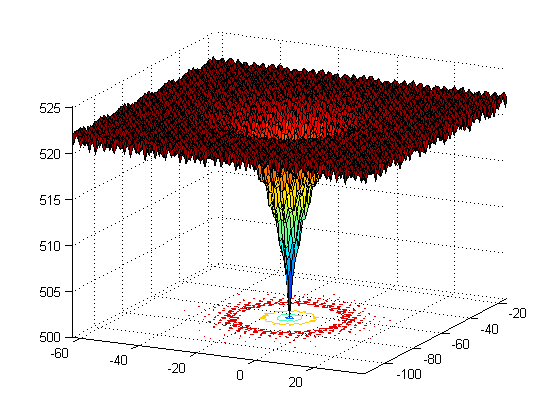
\includegraphics[scale=0.5]{img/f5.png}
    \caption{Mapa 3D para a função \glsentryfull{f5} em duas dimensões. Fonte: \citeonline{cec2014}.}%
    \label{fig:f5}
\end{figure}

\subsection{Configuração dos experimentos}

\todo[author=Gabriel]{Introduzir}

\subsubsection{Constantes}

Dado o escopo do trabalho, foram estabelecidas algumas constantes utilizadas em todos os experimentos realizados, as quais estão listadas na \autoref{tab:constantes}.

\begin{table}[htb]
    \center%
    \begin{tabular}{l l}
        \bottomrule
        \textbf{Constant}    & \textbf{Value} \\ \midrule
        Target               & Min            \\ \midrule
        Population size      & 50             \\ \midrule
        Crossover rate       & 90\%           \\ \midrule
        Mutation             & Flip           \\ \midrule
        Mutation rate        & 5\%            \\ \midrule
        Elitism rate (best)  & 10\%           \\ \midrule
        Elitism rate (worst) & 30\%           \\ \midrule
        Epochs               & 10000          \\ \toprule
    \end{tabular}
    \caption{Constantes utilizadas nos experimentos.}%
    \label{tab:constantes}
\end{table}

Todas as funções tem objetivo de minimização.
Cada gene dos indivíduos da população é representado por um número real entre -100 e 100.
A população inicial é gerada de forma aleatória dentro deste intervalo.
Seu tamanho se mantém fixo ao longo de todas as gerações, em 50 indivíduos.

O operador de \gls{crossover} é aplicado com uma taxa de 90\%, de forma que o método escolhido é parte das variáveis analisadas.
A mutação é aplicada com uma taxa de 5\%, e o método de mutação escolhido é o \texttt{flip}.

O elitismo é aplicado em 10\% dos melhores indivíduos e em 30\% dos piores.
A execução de cada iteração é realizada por 10000 gerações, ou épocas.

\subsection{Variáveis}

As variáveis analisadas nos experimentos se tratam dos operadores de seleção, que podem ser roleta ou torneio --- em que se varia a proporção da população selecionada para participar do torneio (10\%, 20\%, 30\%, 40\%, 50\%) ---, e do operador de \gls{crossover}, que pode ser de um ponto ou aritmético.

A compilação das variáveis resulta em 12 combinações possíveis, que são listadas na \autoref{tab:variaveis}, além das execuções com 10 e 20 dimensões, o que totaliza 24 experimentos para cada função objetivo.

\begin{table}[!ht]
    \center%
    \begin{tabular}{|l|l|l|}
        \bottomrule
        \multirow{2}{*}{Dimensions number} & \multicolumn{2}{l|}{10}                                 \\ \cline{2-3}
                                           & \multicolumn{2}{l|}{20}                                 \\ \hline
        \multirow{6}{*}{Selection}         & \multicolumn{2}{l|}{Roulette}                           \\ \cline{2-3}
                                           & \multicolumn{1}{l|}{\multirow{5}{*}{Tournament}} & 10\% \\ \cline{3-3}
                                           & \multicolumn{1}{l|}{}                            & 20\% \\ \cline{3-3}
                                           & \multicolumn{1}{l|}{}                            & 30\% \\ \cline{3-3}
                                           & \multicolumn{1}{l|}{}                            & 40\% \\ \cline{3-3}
                                           & \multicolumn{1}{l|}{}                            & 50\% \\ \hline
        \multirow{2}{*}{Crossover}         & \multicolumn{2}{l|}{One point}                          \\ \cline{2-3}
                                           & \multicolumn{2}{l|}{Arithmetic}                         \\ \toprule
    \end{tabular}
    \caption{Variáveis analisadas nos experimentos.}%
    \label{tab:variaveis}
\end{table}

Os experimentos foram realizados com 10 execuções para cada combinação de variáveis, a fim de garantir a robustez dos resultados obtidos.
Dessa forma, totaliza 220 execuções para cada função objetivo.


\section{Resultados}%
\label{sec:resultados}

Nesta seção, são apresentados os resultados obtidos a partir da execução dos experimentos descritos na \autoref{sec:metodologia}.

\subsection{Análise dos Resultados}%

A partir dos resultados obtidos, é possível analisar o desempenho dos algoritmos em cada um dos problemas propostos.
Foi considerado o valor de \gls{fitness} do ótimo global ideal como 263.895843.

Com base nos valores de \gls{fitness} das execuções, foram calculados:

\begin{symbols}
    \item[\( \Delta \)] a discrepância em relação ao ótimo global ideal;
    \item[\( \sigma^{2} \)] a variância dos valores de \gls{fitness} obtidos;
    \item[\( \sigma \)] o desvio padrão dos valores de \gls{fitness} obtidos.
\end{symbols}

O experimento consistiu em executar cada algoritmo 10 vezes, variando os pesos atribuídos às penalizações por violação das restrições. Inicialmente, testaram-se pesos de 100, 200, 400 e 800, com o valor dobrando a cada execução. Posteriormente, o peso foi reduzido gradualmente, sendo testados 50, 25, 12,5 e, por fim, 0.

As tabelas~\ref{tab:resultados-genetico} e~\ref{tab:resultados-memetico} apresentam, para os otimizadores \gls{esga} e \gls{oma}, respectivamente, os resultados obtidos.
Elencam-se os valores de \gls{fitness} e de discrepância da melhor solução e da média das 10 execuções realizadas para cada peso de penalização, além de os valores de variância e desvio padrão entre as soluções encontradas.
Os dados completos do experimento com o algoritmo genético%
\footnote{%
    Resultados do experimento para o algoritmo genético. Disponível em: \url{https://docs.google.com/spreadsheets/d/1589Xh2bLunegQypvfnBg_3csuZElcqJtsFiOOzEYmz8/edit?usp=sharing}.
}
e com o memético%
\footnote{%
    Resultados do experimento para o algoritmo memético. Disponível em: \url{https://docs.google.com/spreadsheets/d/1d157cRAJqgtAQ1KfIHSeW07LFzINioJR8bucLpOU43w/edit?usp=drive_link}.
}
estão disponíveis on-line.

\begin{table}[!ht]
    \resizebox{\textwidth}{!}{%
        \begin{tabular}{lrrrrrrr}
            \bottomrule
            \textbf{Weight}                                &
            \textbf{Best fitness}                          &
            \textbf{Average fitness}                       &
            \textbf{Best \(\boldsymbol{\Delta}\)}          &
            \textbf{Average \(\boldsymbol{\Delta}\)}       &
            \textbf{Fitness \( \boldsymbol{\sigma^{2}} \)} &
            \textbf{Fitness \( \boldsymbol{\sigma}\)}
            \\ \midrule
            0                                              &
            \textbf{0.664898658369470}                     &
            \textbf{1.351379134170120}                     &
            261.310316805323000                            &
            262.544463865830000                            &
            0.436608119613905                              &
            0.660763285612862
            \\
            12.5                                           &
            178.997677252294000                            &
            179.104808940107000                            &
            84.504691568419000                             &
            84.791034059893200                             &
            0.013390962925215                              &
            0.115719328226597
            \\
            25                                             &
            216.367732200399000                            &
            216.393958331948000                            &
            47.428849151152000                             &
            47.501884668051500                             &
            0.000845483185771                              &
            0.029077193567664
            \\
            50                                             &
            263.916813724328000                            &
            263.963887551704000                            &
            0.020970724327981                              &
            0.068044551704293                              &
            0.000929526320056                              &
            0.030488134086159
            \\
            100                                            &
            263.907667139552000                            &
            263.929150603033000                            &
            0.011824139552005                              &
            \textbf{0.033307603033092}                     &
            0.000268368246443                              &
            0.016381948798706
            \\
            200                                            &
            263.897546338518000                            &
            263.940946098212000                            &
            \textbf{0.001703338517984}                     &
            0.045103098212383                              &
            0.000428792341542                              &
            0.020707301648019
            \\
            400                                            &
            263.904722244638000                            &
            263.941341028093000                            &
            0.008879244637967                              &
            0.045498028093277                              &
            0.000678108343263                              &
            0.026040513498460
            \\
            800                                            &
            263.901900217279000                            &
            263.931432135312000                            &
            0.006057217278965                              &
            0.035589135312284                              &
            \textbf{0.000207542501157}                     &
            \textbf{0.014406335452058}
            \\ \toprule
        \end{tabular}%
    }
    \caption{Resultados obtidos para o \gls{problem} em que se varia o peso da função de penalização, tendo sido aplicado o otimizador \gls{esga}.
    }%
    \label{tab:resultados-genetico}
\end{table}
\begin{table}[!ht]
    \resizebox{\textwidth}{!}{%
        \begin{tabular}{lrrrrrrr}
            \bottomrule
            \textbf{Weight}                                &
            \textbf{Best fitness}                          &
            \textbf{Average fitness}                       &
            \textbf{Best \(\boldsymbol{\Delta}\)}          &
            \textbf{Average \(\boldsymbol{\Delta}\)}       &
            \textbf{Fitness \( \boldsymbol{\sigma^{2}} \)} &
            \textbf{Fitness \( \boldsymbol{\sigma}\)}
            \\ \midrule
            0                                              &
            \textbf{0.000000000000000}                     &
            \textbf{0.000000000000000}                     &
            263.895843000000000                            &
            263.895843000000000                            &
            \textbf{0.000000000000000}                     &
            \textbf{0.000000000000000}
            \\
            12.5                                           &
            75.000000000000000                             &
            75.000000000000000                             &
            188.895843000000000                            &
            188.895843000000000                            &
            0.000000000000000                              &
            0.000000000000000
            \\
            25                                             &
            150.000000000000000                            &
            150.000000000000000                            &
            113.895843000000000                            &
            113.895843000000000                            &
            0.000000000000000                              &
            0.000000000000000
            \\
            50                                             &
            266.274169979695000                            &
            266.274169979695000                            &
            2.378326979694980                              &
            2.378326979694980                              &
            0.000000000000000                              &
            0.000000000000000
            \\
            100                                            &
            266.274169979695000                            &
            266.274169979695000                            &
            2.378326979694980                              &
            2.378326979694980                              &
            0.000000000000000                              &
            0.000000000000000
            \\
            200                                            &
            266.274169979695000                            &
            266.274169979695000                            &
            2.378326979694980                              &
            2.378326979694980                              &
            0.000000000000000                              &
            0.000000000000000
            \\
            400                                            &
            265.600129207775000                            &
            266.206765902503000                            &
            \textbf{1.704286207775000}                     &
            \textbf{2.310922902502980}                     &
            0.045433096221042                              &
            0.213150407508505
            \\
            800                                            &
            266.274169979695000                            &
            266.274169979695000                            &
            2.378326979694980                              &
            2.378326979694980                              &
            0.000000000000000                              &
            0.000000000000000
            \\ \toprule
        \end{tabular}%
    }
    \caption{Resultados obtidos para o \gls{problem} em que se varia o peso da função de penalização, tendo sido aplicado o otimizador \gls{oma}.
    }%
    \label{tab:resultados-memetico}
\end{table}

Em todas as execuções com pesos iguais ou superiores a 100, o algoritmo genético simples convergiu para soluções muito próximas do ótimo.
O experimento com peso de 100 apresentou uma convergência total antes de 200 gerações, como mostrado na \autoref{fig:ga-weight-100}.
Com pesos de 400, a convergência foi um pouco mais lenta, ocorrendo pouco após 600 gerações, como mostrado na \autoref{fig:ga-weight-400}.

Mesmo com penalizações elevadas, como 800, a convergência se manteve consistente, tendo encontrado uma solução próxima do ótimo global pouco antes da geração 800, como mostrado na \autoref{fig:ga-weight-800}.
Entretanto, com esses pesos mais altos, o algoritmo exigiu um número maior de iterações para alcançar a solução final, embora a qualidade dessa tenha permanecido satisfatória.

\begin{figure}
    \centering
    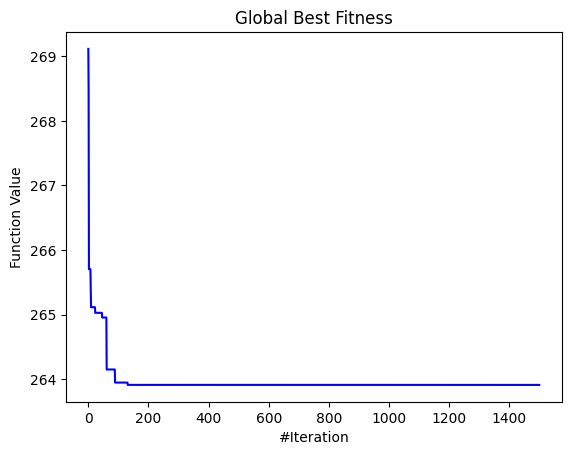
\includegraphics[width=.6\linewidth]{images/weight/100.png}
    \caption{Convergência do algoritmo genético com peso de penalização de 100.}%
    \label{fig:ga-weight-100}
\end{figure}

\begin{figure}
    \centering
    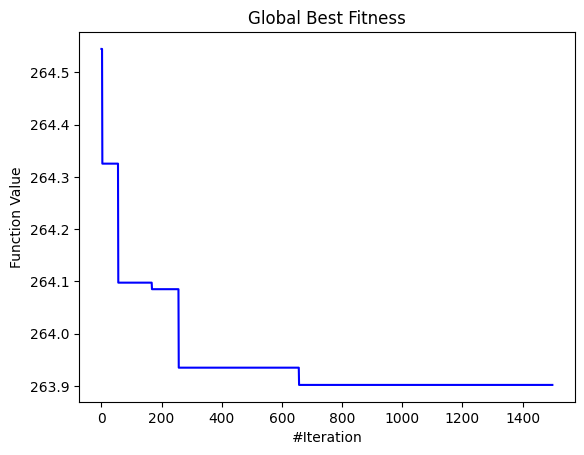
\includegraphics[width=.6\linewidth]{images/weight/400.png}
    \caption{Convergência do algoritmo genético com peso de penalização de 400.}%
    \label{fig:ga-weight-400}
\end{figure}

\begin{figure}
    \centering
    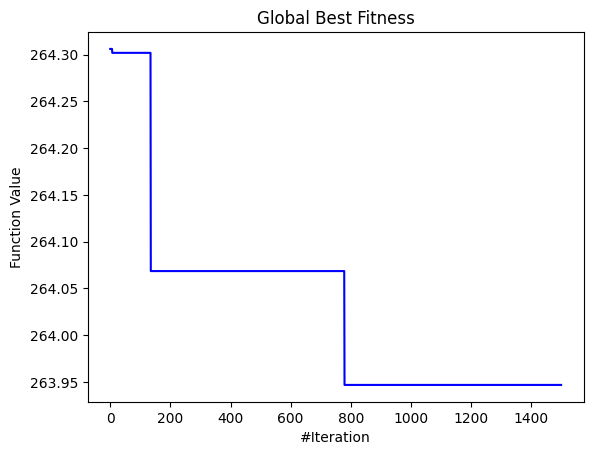
\includegraphics[width=.6\linewidth]{images/weight/800.png}
    \caption{Convergência do algoritmo genético com peso de penalização de 800.}%
    \label{fig:ga-weight-800}
\end{figure}

O algoritmo memético apresentou um desempenho semelhante, atingindo soluções próximas do ótimo em todas as execuções com pesos superiores a 100.
Além disso, sua convergência foi extremamente rápida, sendo que em algumas execuções uma única iteração foi suficiente para encontrar uma solução próxima do ótimo, com um valor aproximadamente uma unidade acima do ideal.

O gráfico do mínimo global poderia parecer sugerir uma estagnação, como mostrado na \autoref{fig:memetic-global}.
Entretanto, através do o gráfico do mínimo local mostrado em \autoref{fig:memetic-local}, é possível constatar que o algoritmo continuou a explorar o espaço de busca com expressiva variabilidade, até o limite de gerações estabelecido.

\begin{figure}
    \centering
    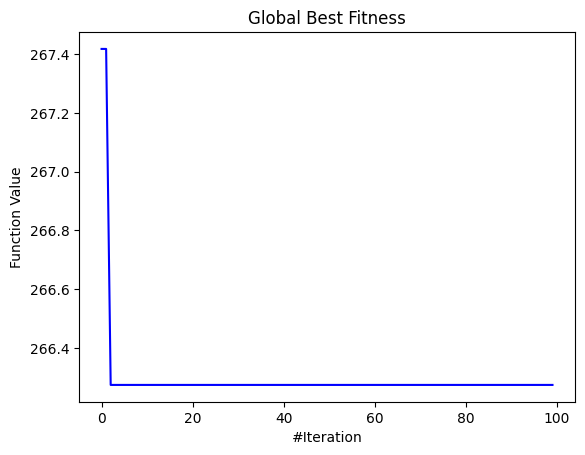
\includegraphics[width=.6\linewidth]{images/convergence/gdbf.png}
    \caption{Convergência do ótimo global para o algoritmo memético.}%
    \label{fig:memetic-global}
\end{figure}

\begin{figure}
    \centering
    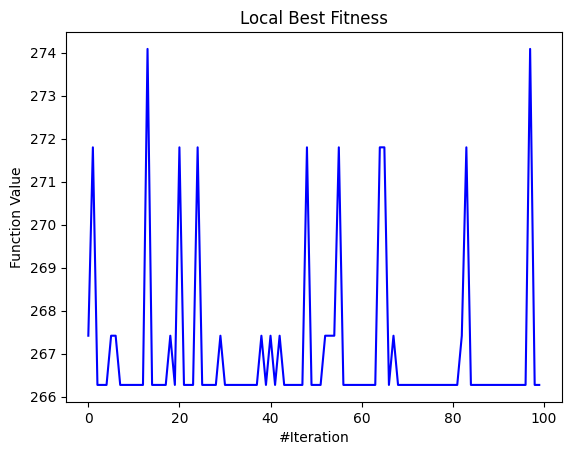
\includegraphics[width=.6\linewidth]{images/convergence/lbfc.png}
    \caption{Convergência do ótimo local para o algoritmo memético.}%
    \label{fig:memetic-local}
\end{figure}

Por outro lado, ao utilizar pesos de penalização mais baixos (50 ou inferiores), ambos os algoritmos começaram a gerar soluções inviáveis, como mostrado nas figuras~\ref{fig:non-viable-ga}, para o algoritmo genético, e~\ref{fig:non-viable-ma}, para o memético.

À medida que o peso diminuía, as soluções aparentavam melhorar em termos de qualidade, mas violavam cada vez mais as restrições, resultando em soluções que estruturalmente são impossíveis.
Comparativamente, o algoritmo memético se comportou de forma mais agressiva, gerando soluções inviáveis mais rapidamente que o algoritmo genético simples.

\begin{figure}
    \centering
    \begin{subfigure}{.5\textwidth}
        \centering
        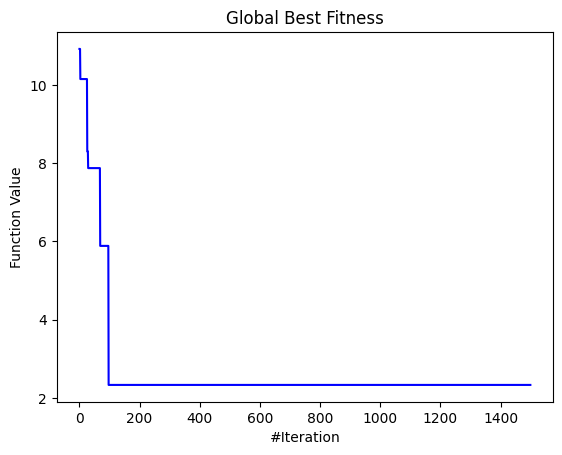
\includegraphics[width=1\linewidth]{images/non_viable/0/GA.png}
        \caption{Peso 0.}
    \end{subfigure}%
    \begin{subfigure}{.5\textwidth}
        \centering
        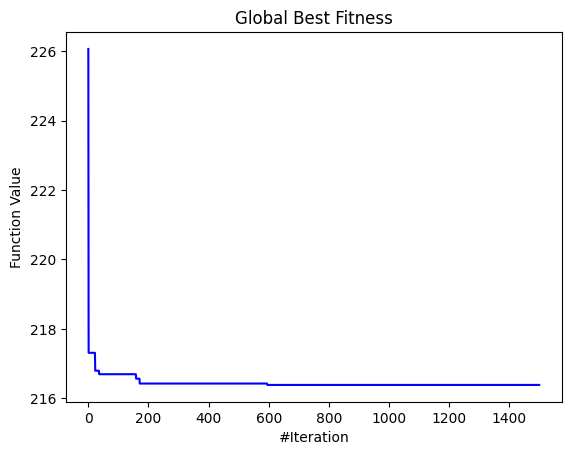
\includegraphics[width=1\linewidth]{images/non_viable/25/GA.png}
        \caption{Peso 25.}
    \end{subfigure}%
    \caption{Soluções inviáveis geradas pelo algoritmo genético.}%
    \label{fig:non-viable-ga}
\end{figure}

\begin{figure}
    \centering
    \begin{subfigure}{.5\textwidth}
        \centering
        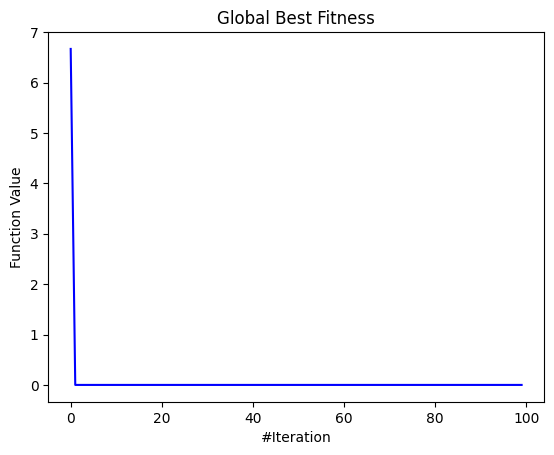
\includegraphics[width=1\linewidth]{images/non_viable/0/MA.png}
        \caption{Peso 0.}
    \end{subfigure}%
    \begin{subfigure}{.5\textwidth}
        \centering
        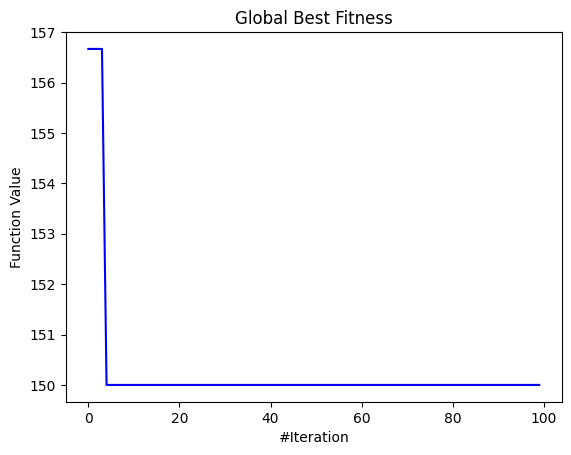
\includegraphics[width=1\linewidth]{images/non_viable/25/MA.png}
        \caption{Peso 25.}
    \end{subfigure}%
    \caption{Soluções inviáveis geradas pelo algoritmo memético.}%
    \label{fig:non-viable-ma}
\end{figure}


\section{Conclusão}%
\label{sec:conclusao}

Os resultados obtidos neste experimento evidenciam tanto as limitações quanto os potenciais do algoritmo genético quando aplicado às funções \gls{f1} e \gls{f5}. No caso da função \gls{f1}, observamos que os resultados ficaram significativamente piores do que o ótimo global, indicando que a mutação utilizada, mesmo com uma taxa de 5\%, não foi suficiente para explorar o espaço de busca de forma satisfatória. Isso sugere que o algoritmo pode ter convergido prematuramente para ótimos locais. No entanto, além da mutação, outros fatores podem ter contribuído para o desempenho insatisfatório, como a própria natureza do algoritmo genético, que pode não ser ideal para otimizar funções convexas como \gls{f1}.

Por outro lado, a função \gls{f5}, que possui uma topologia não convexa e mais íngreme, obteve resultados muito próximos do ótimo global. Isso sugere que o algoritmo genético é particularmente eficaz para este tipo de função, onde a exploração e os saltos no espaço de busca são mais facilmente capturados e otimizados.

Esses resultados ressaltam a importância de se considerar a adequação do algoritmo ao tipo de função a ser otimizada. Em algumas situações, como no caso da função \gls{f1}, o algoritmo genético pode não ser a melhor escolha, enquanto para funções como \gls{f5}, ele se mostra bastante eficiente. Essa conclusão aponta para a necessidade de uma análise cuidadosa na seleção de algoritmos de otimização, levando em conta tanto os operadores quanto a natureza das funções envolvidas.
% =====

% =====
% ELEMENTOS PÓS-TEXTUAIS
% =====
\postextual{}

% --- Referências ---
\bibliography{bibliography}

% --- Glossário ---
\printglossary[type=main,style=altlist,title=Glossário]
\printglossary[type=acronym,style=altlist,title=Lista de Abreviaturas e Siglas]
% =====

\end{document}